%\documentclass{acm-book-v2}
%\RequirePackage[errorshow]{tracefnt}
%\newcommand{\mpage}[1]{}
%\newcommand{\indexfn}[1]{}

%\usepackage{showframe}

%\usepackage{custom-tooltip}
%\usepackage{custom-tooltip-Alt-Text-View}

%\usepackage{wrapfig}

%\begin{document}


\addchap{\label{chap:Bio}Author's Biography}


\section*{Domenico Talia}\label{DomenicoTalia}
\begin{wrapfigure}[13]{l}{0.3\textwidth}
\vspace*{-16.5pt}
\tooltipZFour{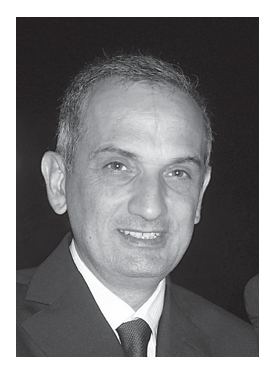
\includegraphics{graphics/Author_Bio/Domenico_Talia.eps}}{Photo of Domenico Talia.}[-130pt,23pt]
\vspace*{-18.5pt}
\end{wrapfigure} \textbf{Domenico Talia} is a full professor of computer engineering at the University of Calabria, Italy and an honorary professor at Amity University, Noida, India. He is co-founder of DtoK Lab. His research interests include Big Data analysis, cloud computing, machine learning, social data mining, parallel and distributed data analysis, mobile computing, and parallel programming.

He has published 12 books and more than 400 papers in archival journals such as \textit{CACM}, \hbox{\textit{Computer},} \textit{IEEE TKDE}, \textit{IEEE TSE}, \textit{IEEE TPDS}, \textit{IEEE} \textit{TSMC-B}, \textit{IEEE Micro}, \textit{ACM Computing Surveys}, \textit{FGCS}, \textit{\hbox{Parallel} \hbox{Computing}}, \textit{IEEE Internet Computing}, and international conference proceedings. He is a member of the editorial boards of \hbox{\textit{Computer},} \textit{IEEE Transactions on Parallel and Distributed Systems}, \textit{ACM Computing Surveys}, \textit{Future Generation Computer Systems}, \textit{Journal of Cloud Computing}, \textit{International\break Journal of Web and Grid Services}, \textit{Big Data and Cognitive Computing}, and \textit{Multiagent and Grid Systems}.

Prof. Talia has served as chair, organizer, or program committee member of several international conferences and given many invited talks, tutorials, and seminars in conferences and schools. He is a senior member of the ACM and IEEE.

A list of publications can be found here: \href{https://scholar.google.it/citations?user=domenicotalia}{https://{\allowbreak}scholar.{\allowbreak}google.it/{\allowbreak}citations?{\allowbreak}user={\allowbreak}domenicotalia}.



%\end{document}

